\documentclass[twoside,11pt,english]{article}


% ------
% Fonts and typesetting settings
\usepackage[sc]{mathpazo}
\usepackage[T1]{fontenc}
\linespread{1.05} % Palatino needs more space between lines
\usepackage{microtype}
\usepackage{babel}
\usepackage{graphicx}

% ------
% Page layout
\usepackage[hmarginratio=1:1,top=32mm,columnsep=20pt]{geometry}
\usepackage[font=it]{caption}
\usepackage{paralist}
\usepackage{multicol}

% ------
% Abstract
\usepackage{abstract}
	\renewcommand{\abstractnamefont}{\normalfont\bfseries}
	\renewcommand{\abstracttextfont}{\normalfont\small\itshape}


% ------
% Titling (section/subsection)
\usepackage{titlesec}
\renewcommand\thesection{\Roman{section}}
\titleformat{\section}[block]{\large\scshape\centering}{\thesection.}{1em}{}


% ------
% Header/footer
\usepackage{fancyhdr}
	\pagestyle{fancy}
	\fancyhead{}
	\fancyfoot{}
	\fancyhead[C]{}
	\fancyfoot[RO,LE]{\thepage}


% ------
% Clickable URLs (optional)
\usepackage{hyperref}

% ------
% Maketitle metadata
\title{\vspace{-15mm}%
	\fontsize{24pt}{10pt}\selectfont
	\textbf{Factoring large integers using Quadratic Sieve}
	}	
\author{%
	\large
	\textsc{Christopher Teljstedt} \\[2mm]
	\normalsize	\href{mailto:chte@kth.se}{chte@kth.se} 
	\and
	\textsc{Henrik Viksten} \\[2mm]
	\normalsize	\href{mailto:hviksten@kth.se}{hviksten@kth.se}
	}

% ------
% Macros
\providecommand{\myceil}[1]{\left \lceil #1 \right \rceil }
\providecommand{\myfloor}[1]{\left \lfloor #1 \right \rfloor }

%%%%%%%%%%%%%%%%%%%%%%%%
\begin{document}

\maketitle
\thispagestyle{fancy}


\begin{abstract}
\noindent Suspendisse id urna vel risus venenatis ultrices ut vel odio. Donec aliquet est at magna tincidunt ut rutrum lacus cursus. Praesent ultricies aliquam erat quis scelerisque. Vestibulum interdum interdum augue, at placerat turpis tempus nec. Vestibulum feugiat, tellus ultrices tempor fermentum, ipsum dolor vestibulum eros, sed vulputate felis eros eget ipsum. Fusce ultricies dapibus turpis non pretium. Suspendisse potenti. Integer porttitor, lorem ac mattis fermentum, metus neque scelerisque sapien, vel lobortis orci erat at sapien. 
\end{abstract}
	

\begin{multicols}{2}
\section{Introduction}
This report will cover the work of a integer factorization program written in the course DD2440 advanced algorithms. Methods that can be used to solve the integer factorization problem in a effective way using existing algorithms and an explanation of methods used.

\subsection{Purpose}
The goal of the program is to pass kattis test cases with as high score as possible, this is done by improving the program step-by-step and gradually increasing the performance. In the report the methods used will be analyzed. How they work independently and their correlation in our implementation.

\subsection{Problem}
An unknown set of 100 integers in varying size are used as input to the algorithm from kattis. The output is either the factors of the input in case it is solved or the string fail otherwise. One of the problems is dealing with large integers within the timeframe but also finding every single non-trivial factor. The restrictions in kattis are 15 seconds and 64MB of memory.

\subsection{Scope}
There is no intention of reinventing any methods that already exists, the idea is to create a solver that can factorize unknown integers and in the end get a high score on kattis.

\subsection{Statement of Collaboration}
Some text.
\newpage
\section{Preliminaries}
{\bf Notation.} By 'log$_b$' we denote the base $b$ logarithm and the natural logarithm denotes by ln=log$_e$ with $e \approx 2.71828$. 
The largest integer $\leq x$ is denoted by '[x]'.  The number of primes $\leq x$ is denoted by '$\pi(x)$', and due the \emph{Prime number theorem}\cite{Hardy2008}
we know that $\pi(x) \approx x / $ln$(x)$ .

{\bf Smoothness.} A positive integer is \emph{B-smooth} if all its prime factors are lesser than a boundary $B$.
Furthermore an integer, say $x$, is said to be \emph{smooth with respect to S}, if $x$ can be completely factored using
integers by some set $S$ alone.


{\bf Modular arithmetic.} Throughout this paper '$x \equiv y$ mod $n$' means that $(x-y)$ is a multiple of $n$ whereas $x,y$ and $n \in \mathbb{N}_{\ne 0}$.

Similarly, '$x \not\equiv y$ mod $n$' mean that $(x-y)$ is not a multiple of $n$. 
Euclid's algorithm for finding the \emph{greatest common divisor} of two non-negative integers, say x and z, is denoted by gcd$(x,z)$.

\newpage
\section{Quadratic Sieve}
\subsection{Brief explaination}
The quadratic sieve algorithm is today the algorithm of choice when factoring very large composite numbers
with no small factors. The general idea behind quadratic factoring is based on Fermat's observation that
a composite number $n$ can be factored if one can find two find two integers $x,y \in Z$, such
that $x^2 \equiv x^2$ (mod $n$) and $x \not\equiv \pm y$ (mod $n$). This would imply that,
\begin{equation}
n \ | \ x^2-y^2 = (x-y) \cdot (x+y)
\end{equation}
but $n$ neither divides $(x-y)$ nor $(x+y)$. 
Furthermore it can be rewritten as $(x-y) \cdot (x+y) = k \cdot p \cdot q$ for some integer $k$, thus becoming two possible cases.

\begin{itemize}
	\item either $p$ divides $(x-y)$ and $q$ divides $(x+y)$, or vice versa.
	\item or both $p$ and $q$ divides $(x-y)$ and neither of them divides $(x+y)$, or vice versa.
\end{itemize}

Hence, the greatest common divisor of ($x-y,n$) and ($x+y,n$) would in first case yield $p$ or $q$ and a non-trivial factor of 
$n$ is found. In the second case we get $n$ or $1$ and trivial solution is found. 

Carl Pomerance suggested a method to find such squares\cite{Pomerance1985}. The first step in doing so is to is to define the polynomial 
\begin{equation}
q(x) = (x + \myfloor{\sqrt{n}})^2-n 
\end{equation}
One might realize that this satisfies the relation $(x + \myfloor{\sqrt{n}})^2 \equiv q(x) \ (\textrm{mod} \ n)$.

Now, consider we have integers $x_1, x_2, \ldots, x_k$ for which so that the product $q(x_1) \cdot q(x_1) \cdot \ldots \cdot q(x_n)$
is a perfect square, and call it $y^2$. Then if we let $x = (x_1 + \myfloor{\sqrt{n}})\cdot(x_2 + \myfloor{\sqrt{n}})\ldots(x_k + \myfloor{\sqrt{n}})$
we have a solution $x^2 \equiv y^2$ that satisfies equation (1).

To find such $x$'s we must realize that we if a prime $p$ divides $q(x_i)$ then $(x_1 + \myfloor{\sqrt{n}})^2 \equiv n$ (mod $p$).
Hence, $n$ is a quadratic residue modulo $p$ and we only need to consider those primes. Thus the set of primes $p_i$ for which the Legendre symbol $(\frac{n}{p_i})$ is 1. This set of primes is a tool for factoring which we will further on referr as $factor \ base$.

Lets consider a factor base $P$ with the primes $p_1, p_2, ..., p_k$ that is $k \leq B$ and coprime to $n$.
We want to find small $x_i$ so that $q(x_i)$ is smooth in respect to $P$. If we find such $x$'s we say that $q(x_i) = (x + \myfloor{\sqrt{n}})^2-n$
is B-smooth and we can factor $y^2$ completely over the factor base.

A prime factorization $p_1^{a_1} \cdot p_2^{a_2} \cdot \ldots \cdot p_k^{a_{\pi(B)}}$ of a B-smooth number $v$ can then be expressed as,
we can express as a exponent vector $e(v) = (a_1, a_2, \ldots, a_{\pi(B)})$ and we arrive at following formula.

\begin{equation}
y^2 \equiv \prod_{i=1}^{\pi(B)} p_i^{e_i{v}}
\end{equation}

Then the product of subsequence of $v$ i.e. $q(x_1) \cdot q(x_2) \cdot \ldots \cdot q(x_k)$ produced a 
square $iff$ the exponent vectors has only even entries. The linear combinations producing 
a perfect square can the be solved with Gaussian Eliminations modulo 2 if the exponent vectors
is represented as the rows of a matrix. Thus, the column sums must be even.

\subsection{Brief explaination}
\newpage
\section{Background}
As described in the scope the intention is not to find a new method of factoring integers but instead use existing methods and implement them in a intelligent way.

\subsection{Trial Division}
Trial division is an easy implemented algorithm for finding factors to $N$. Like its name suggests it uses tries to divide $N$ by using a $x > 2$. If the remainder of $N/x = 0$ the factor is a non-trivial factor, if we cannot find a divisor $x$ that gives the remainder $0$ then $N$ is a prime.

The restrictions for the algorithm are easy to find and improve, $N > 1$ and $x > 2$. This can be improved by saying that $N > x$ and since the factors of N cannot be larger than $\sqrt{N}$ we can also say that $\sqrt{N} > x > 2$. Another improvement is to only do tests when $x$ is a prime number. Although trial division is easy to implement and guaranteed to grant an answer it is not efficient for large a $N$.

\subsection{Pollard's Rho}
Pollard rho is a prime factorization algorithm which is based on Floyd’s cycle-finding algorithm. The idea of pollard rho algorithm is to iterate a formula until it falls into a cycle. We want to find a $x$ and $y$ where the $x$ makes twice as many iterations as the $y$ using a function $modulo N$ as a generator of a pseudo-random sequence. The $GCD|x - y|$ of $N$ is taken each step, and the GCD reaches $N$ we have not found an answer and the algorithm terminates with a failure.

We can write $N = p * q$, when $x$, which iterates twice as fast as $y$, catches up with $y$ which will happen eventually, at this point factor $p$ will be found. The time it will take cannot be proven matematically and can only be proven by heuristics. If the sequence behaves randomly it would take approximately p steps to find p, which is not very effcient. \cite{avalg} \\

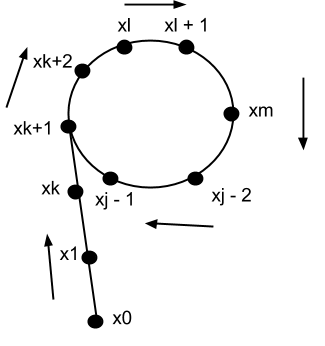
\includegraphics[scale = 0.5]{pollards.png}

The figure above illustrates the Pollard's Rho cycle. The mapping of $x_{i+1}$ is instead replaced with a function $x^2+1$ so that we get $x^2_{i}+1$  $mod$ $N$ the factor $p$ will be found after $O(\sqrt{p})$  $\epsilon$ $O(N^{1/4})$ steps. \cite{avalg}\\

Pollard's rho algorithm can be improved further by implementing Brent's cycle finding method. \cite{brent}

\subsection{Miller-Rabin primality test}
Miller-Rabin primality test is a probabalistics algorithm which determines if the given input $N$ is a prime. It is based on the properties of strong pseudoprimes, given an integer $N$, $N = 2^r * s + 1$ where $s$ is odd you choose a random number $a$ with the properties $1 \leq a \leq N - 1$. When $a^s \equiv 1$ $mod$ $N$ or $a^{2js} \equiv - 1$ $mod$ $N$ where $0 \leq j \leq r - 1$, if the input number $N$ is a prime it will pass the test with any random number $a$.

Since Miller-Rabin is a probabalistics method it is not completely true that $N$ is a prime simply by passing the test, however the probability that the answer is true when $N$ is a composite number is $1 / 4^{N}$ which grows quickly with $N$. It can be considered a very small trade-off to use a probabalistics method because the algorithm executes at $O(k log^3 N$ where $k$ is the number of different values of $a$ tested. \cite{miller}
\newpage
\section{Implementation}

For our implementation we used several papers as reference. One that really come handy
lecture notes by Carl Pomerance \cite{Pomerance05smoothnumbers}. We implemented a naive
quadratic sieve using only single polynomial paradigm.

The program can be divided into three general phases:
\begin{itemize}
\item calculating smoothness bound and generate factor base
\item sieving
\item gaussian elimination
\end{itemize}

\newpage
\section{Results}
These tests were solely based on the score and running time on the 
\texttt{KATTIS} problem \texttt{oldkattis:factoring}.

\paragraph{Primality testing}
At first we just tried to do a primality test with Miller-Rabin. 
The results can be seen in table

 \textbf{Score} 1   \textbf{Running time} 0.01s 
                          

\paragraph{Quadratic sieve}

We implemented a naive Quadratic Sieve from start and
at first with bad B smooth boundary. It had
unoptmizied sieving functions, we did handle perfect powers.

This yielded a result on Kattis as shown below.

 \textbf{Score} 85   \textbf{Running time} 13.56s 
                          

By improving on the problems mentioned above and tweaking the smoothness boundary
B which regulates the factor base size aswell as the number of linear relations,
i.e how many extra smooth numbers, we managed to get 100 points score on Kattis.

 \textbf{Score} 100   \textbf{Running time} 4.32s 

\subsection{Kattis submission}
The best Kattis submission has the ID:459013.
\newpage
\section{Discussion}
We chose to work with quadratic sieve since it's one of the most efficient integer factorization algorithms out there. It is the fastest algorithm for factorization up to 100 bit integers, the challenge was obvious but since we had knowledge that Pollard's Rho combined with Brent's cycle finding granted approximately 75 points in KATTIS and that the code was not a big challenge to write we wanted to give ourselves a challenge and dive in to a front-running algorithm.
The result was as expected from a correctly implemented quadratic sieve method, however, on the first submitt (that was working) we got a score of 85 points which was due to partly a lack of general optimization but the main reason was making sure the smoothness bounds worked correctly. There are a lot of mathematical parts to implementing this algorithm, altough not very complex math in theory getting all the parts of the algorithm to work well was a tough job. The understanding of the concept came as we went along and step-by-step we improved our code and realized the earlier errors we made and in the end realized that the concept is not hard to graps if you divide the problem in to subproblems and follow pre-existing formulas to execute it.
\newpage
\section{Conclusion}
In hindsight there is no regret of choosing the more complex solution to the problem, it did not only give us more understanding of how to solve the problem we were given in an intelligent way but we also managed to successfully implement the quadratic sieve algorithm to achieve maximum score in KATTIS. Of course the solution can be optimized further but considering the time constraints we are satisfied with our work.

\newpage
\bibliographystyle{plain}
\bibliography{References}
\end{multicols}

\end{document}
